% Drawing 74/07-9 -- folder 74, batch 07, archive page 133 (PDF page 134).
% Transcription: un cube en perspective, une face en traits épais, des arêtes en pointillé.
% Kind: cube in perspective. Method 2 (schematic redraw from the facsimile). Status: partial.
% Notes: A cube: one face in thick strokes, the other edges in dotted strokes forming the outline, crossing diagonals inside. The dotted strokes are approximate.
% Coordinates: 1 unit = 1 mm = 1/100 of the crop width (bbox in page fractions: [0.54, 0.41, 0.68, 0.48]).
% Redrawn by Claude (claude-opus-5-5), issue #73, 2026-11-07; not checked by a human; not compiled (no TeX in the session).
% Rights: reproduces part of the work -- behind RENDER_TRANSCRIPTS, never published by itself.
\documentclass[tikz,border=3pt]{standalone}
\usepackage{amsmath,amssymb}
\usetikzlibrary{patterns,arrows.meta}
\tikzset{pencil/.style={black!45}, struck/.style={black!35}, mark/.style={circle,draw,inner sep=1.3pt}, pt/.style={circle,fill,inner sep=0.9pt}, opt/.style={circle,draw,fill=white,inner sep=1.1pt}}
\begin{document}
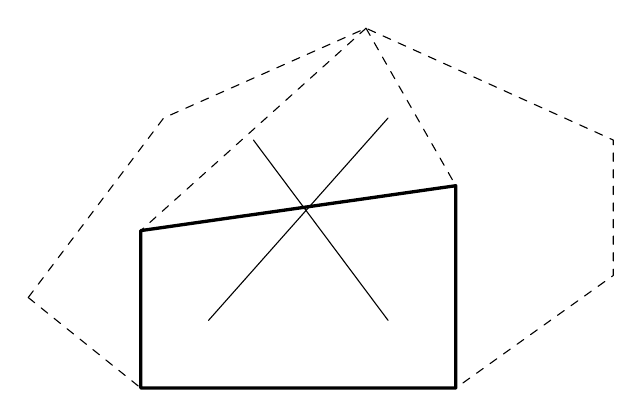
\begin{tikzpicture}[x=1mm,y=1mm,line cap=round,line join=round,font=\scriptsize]
\draw[very thick] (25.7,-38.5) -- (65.7,-32.8) -- (65.7,-58.5) -- (25.7,-58.5) -- cycle;
\draw[dashed] (11.4,-47) -- (28.6,-24.2) -- (54.3,-12.8) -- (85.7,-27) -- (85.7,-44.2) -- (65.7,-58.5);
\draw[dashed] (11.4,-47) -- (25.7,-58.5);
\draw[dashed] (54.3,-12.8) -- (25.7,-38.5);
\draw[dashed] (54.3,-12.8) -- (65.7,-32.8);
\draw (40,-27) -- (57.1,-49.9);
\draw (57.1,-24.2) -- (34.3,-49.9);
\end{tikzpicture}
\end{document}
